\chapter{Introduction}
\label{ch:introduction}

\section{Motivation}
\section{Geometry Description}
  \label{sec:geometry_description}
  % include can figure

  \begin{figure}
    \centering
    \includegraphics[width=\textwidth]{reactor_materials}
    \caption{Example of Sodium-cooled Fast Reactor based on MONJU.}
    \label{fig:reactor_materials}
  \end{figure}

  In a cross-sectional assembly view, dimensions are presented in
  \fref{fig:pin_model} and \fref{fig:hex_can}. In \fref{fig:hex_can}, $Th_{Box}$
  is the thickness of the assembly box, F2F is the flat-to-flat measurement of
  the outside of the hexagonal can, and Pitch is the distance between the
  center of two pins. In future notation, the quantity ``Pitch'' is also denoted
  $S$. Using the geometry described in these figures, the material
  cross-sectional areas are calculated according to the given formulae where
  $N_{pin}$ is the number of pins in the assembly.
  \begin{align}
    \label{eq:afrac_first}
    A_{total} &= \frac{\sqrt{3}}{2} F2F^2 \\
    A_{can} &= A_{total} - 
      \frac{\sqrt{3}}{2} \left(  F2F - 2 \, Th_{Box} \right) \\
    A_{wrap} &= N_{pin} \frac{\pi}{4} D_{wrap}^2 \\
    A_{clad} &= N_{pin} \pi (R_C^2 - R_B^2) \\
    A_{bond} &= N_{pin} \pi (R_B^2 - R_F^2) \\
    A_{fuel} &= N_{pin} \pi R_F^2 \\
    \label{eq:afrac_last}
    A_{cool} &= A_{total} - A_{can} - A_{wrap} - A_{clad} - A_{bond} - A_{fuel}
  \end{align}
  Calculating the areas as above allows for calculation of cross-sectional area
  fractions. Assuming constant dimensions within an element in the axial
  direction, these area fractions are equivalent to volume fractions and are
  useful for neutron cross-section calculations. Additionally, these formulae
  allow for thermal expansion calculations as the liquid sodium in the bond and
  the coolant are allowed to vary to allow for the expansion of other materials.

  \begin{figure}
    \centering
    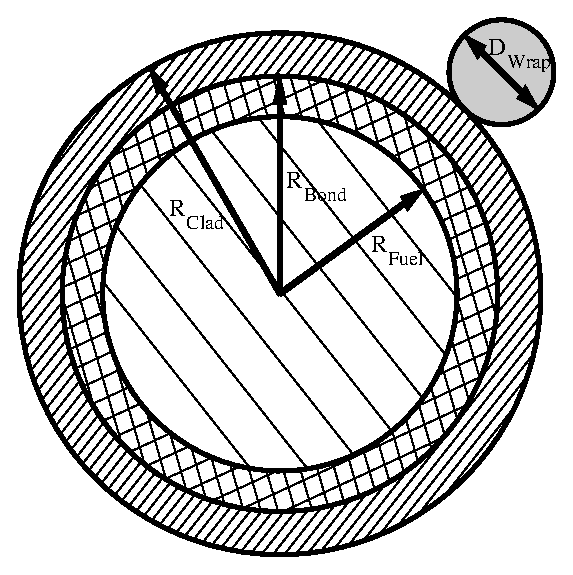
\includegraphics[width=0.5\textwidth]{pin_model}
    \caption{Dimensions of Thermal Hydraulic Pin Model.}
    \label{fig:pin_model}
  \end{figure}

  \begin{figure}
    \centering
    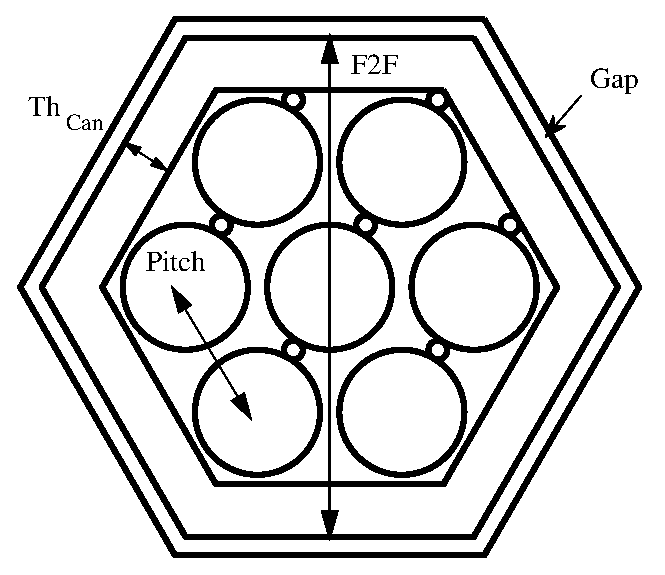
\includegraphics[width=0.5\textwidth]{hex_can}
    \caption{Dimensions of Hexagonal Can.}
    \label{fig:hex_can}
  \end{figure}

\section{Cross Section Generation}
